\setcounter{secnumdepth}{2}

\chapter{Description of the problem}

\section{Prerequisites and used notations}

In order to understand the following chapters, it is needed to (re)introduce some useful notations that are widely used in the context of graph theory \cite{graphtheory}.


\subsection{The different definitions of graphs}

In the context of discrete mathematics, a \textit{graph} $G = (V, E)$ is a set $V$ of objects, called \textit{vertices}, and a set $E$ of tuples (or pairs) between these vertices, called \textit{edges}. The notations $V(G)$ and $E(G)$ denote the set of vertices and the set of edges of $G$ respectively. Graph theorists distinguish different types of graphs. The following definitions cover the graphs that will be used in the context of this master thesis.

\begin{definition}[Simple graph]
    \label{def:simple_graph}
    A graph $G$ is said to be \textit{simple} if it has maximum one edge between each pair of its vertices. Furthermore, a simple graph has no edge that begins and ends at the same vertex.
\end{definition}

\begin{definition}[Undirected graph]
    \label{def:undirected_graph}
    A graph $G$ is said to be \textit{undirected} if $E(G)$ is a set of unordered pairs, i.e. if its edges are bidirectional. It is opposed to the concept of \textit{directed graphs}, in which the edges are ordered tuples.
\end{definition}

\begin{definition}[Edge-coloured graph]
    \label{def:edge_coloured_graph}
    An \textit{edge-colouring} $k$ of a graph $G$ is a function that maps each edge $e \in E(G)$ to a colour $k(e)$ (often represented as an unsigned integer). An \textit{edge-coloured graph} $G_k$ is a graph $G$ equipped with an edge-colouring $k$.
\end{definition}

\begin{definition}[Mixed edge-coloured graph]
    \label{def:mixed_edge_coloured_graph}
    An \textit{mixed edge-colouring} $k$ of a graph $G$ is a function that maps each edge $e = (v_1, v_2) \in E(G)$ to 2 colours $k(e, v_1)$ and $k(e, v_2)$ (often represented as unsigned integers). An \textit{mixed edge-coloured graph} $G_k$ is a graph $G$ equipped with a mixed edge-colouring $k$.
\end{definition}

\begin{definition}[Weighted graph]
    \label{def:weighted_graph}
    A \textit{weight attribution} $w$ of a graph $G$ is a function that maps each edge $e \in E(G)$ to a weight $w(e)$. Most often, this weight is assumed to be a real number. But in the context of this master thesis, this weight is a complex number. A \textit{weighted graph} $G^w$ is a graph $G$ equipped with a weight attribution $w$.
\end{definition}


\subsection{Paths and connectivity concepts}

\begin{definition}[Path]
    \label{def:path}
    Given a graph $G$, a \textit{path} $P = (e_1, e_2, \dots, e_l)$ is an ordered sequence of different edges from $E(G)$ respecting the following property.
    \begin{center}
        $e_i[2] = e_{i + 1}[1] \forall i \in [1, l - 1]$
    \end{center}
\end{definition}

\begin{definition}[Hamiltonian path]
    \label{def:hamiltonian_path}
    A path $H$ of a graph $G$ is said to be \textit{Hamiltonian} if
    \begin{center}
        $\left\{
        \begin{tabular}{l}
            All the vertices in $V(G)$ appear in $H$ and \\
            $H$ begins and ends at the same vertex.
        \end{tabular}
        \right.$
    \end{center}
\end{definition}

\begin{definition}[Arc of Hamiltonian cycle]
    \label{def:arc}
    Let $G$ be a graph that admits a Hamiltonian cycle $H = (v_1, v_2, \dots, v_n)$. In the context of this master thesis, what is called the \textit{arc} from $v_i$ to $v_j$ on $H$, denoted by $H_{i, j}$, is defined as follow.
    
    \begin{center}
        $H_{i, j} = \left\{
        \begin{array}{l l}
            \left\{
                \{v_i, v_{i+1}\}, \{v_{i+1}, v_{i+2}\}, \dots, \{v_{j-1}, v_j\}
            \right\} & \mbox{ if } i < j \\
            \left\{
                \{v_i, v_{i+1}\}, \{v_{i+1}, v_{i+2}\}, \dots, \{v_n - 1, v_n\},  \{v_n, v_1\}, \{v_1, v_2\}, \dots, \{v_{j-1}, v_j\}
            \right\} & \mbox{ if } j < i \\
            \left\{\right\} & \mbox{ if } i = j
        \end{array}
        \right.$
    \end{center}
    
    In other words, $H_{i, j}$ is the set of edges that builds the path from $v_i$ to $v_j$ along $H$ when being allowed to go only in the positive direction. An example is shown in figure \ref{fig:H_i_j}.

    \begin{figure}[H]
        \ctikzfig{figures/problem_presentation/definitions/H_i_j}
        \caption{Visualisation of the arc $H_{5, 2}$ on a Hamiltonian path $H$ of some graph $G$ from $v_5$ to $v_2$. The arc is marked using thicker edges.}
        \label{fig:H_i_j}
    \end{figure}
    
\end{definition}

\begin{definition}[Connected graph]
    \label{def:connected_graph}
    A graph $G$ is said to be \textit{connected} if $\forall v_1, v_2 \in V(G), \exists$ a path $P$ between $v_1$ and $v_2$ in $G$. If this property is not satisfied, then $G$ is \textit{disconnected}.
\end{definition}

\begin{definition}[Edge connectivity]
    \label{def:edge_connectivity}
    The \textit{edge connectivity} of a graph $G$ is the minimum number of edges we have to remove from $E(G)$ to make it disconnected.
\end{definition}

\begin{definition}[Maximum and minimum degree]
    \label{def:degree}
    The \textit{degree} of a vertex $v$ in a graph $G$, denoted $d(v)$, is the number of edges touching $v$ in $E(G)$. The \textit{minimum degree} of $G$, denoted $\delta(G)$, and the \textit{maximum degree} of $G$, denoted $\Delta(G)$, are defined as follow
    \begin{center}
        $\left\{
        \begin{array}{l}
            \delta(G) = \min\limits_{v \in V(G)} d(v)\\
            \Delta(G) = \max\limits_{v \in V(G)} d(v)
        \end{array}
        \right.$
    \end{center}
\end{definition}


\subsection{Matchings definitions and notations}

The studied problem in this master thesis is centered about the (non)existence of matchings in specific graphs. For this reason, the matchings-related concepts are (re)defined here. \cite{graphtheory}

\begin{definition}[Matching]
    \label{def:matching}
    Given a graph $G$, two edges from $E(G)$ are said to be \textit{independent} if they do not contain any vertex in common. A \textit{matching} $M$ of $G$ is a set of independent edges of $E(G)$. 
\end{definition}

\begin{definition}[Perfect matching]
    \label{def:perfect_matching}
    A matching $M$ of a graph $G$ is said to be \textit{perfect} if it covers the whole set of $G$'s vertices, i.e. if every vertex $v \in V(G)$ appears in one of the edges of $M$.
\end{definition}



\section{Simplified version of the conjecture (solved)}

The following statements and definitions directly come from Mario Krenn's formulation of the problem in \cite{wordpress}. He first defines the notion of monochromatic graphs, followed by the notion of its matching index.

\begin{definition}[Monochromatic graph]
    \label{def:monochromatic_graph}
    An edge-coloured graph $G_k$ is said to be \textit{monochromatic} if all its perfect matchings are monochromatic, i.e. for all perfect matchings $M$, the edges of $M$ are all of the same colour.
\end{definition}

An example of monochromatic graph is shown in Figure \ref{fig:k4_pm}.

\begin{definition}[Matching index]
    \label{def:matching_index}
    Let $G$ be a graph. For any edge-colouring $k$ such that $G_k$ is monochromatic, let $c(G, k)$ be defined as the number of different colour classes containing at least one perfect matching of $G_k$. The \textit{matching index} of $G$, denoted $c(G)$, is the maximum value that $c(G, k)$ can take.
    \begin{center}
        $c(G) = \max\limits_{k \in \mathcal{K}(G)}(c(G, k))$
    \end{center}
    where $\mathcal{K}(G)$ describes here the set of all possible edges-colourings $k$ of $G$ such that $G_{k}$ is monochromatic.
\end{definition}

\begin{figure}[H]
    \ctikzfig{figures/problem_presentation/simplified/k4_pm}
    \caption{Example of monochromatic graph : an edge coloured version of $K_4$. It has maximum 3 monochromatic perfect matchings of different colours. Therefore, $c(K_4) = 3$.}
    \label{fig:k4_pm}
\end{figure}

Equipped with these concepts, the reader has now all the knowledge to understand the simplified version of the conjecture.

\begin{theorem}[Simplified version of Krenn's conjecture]
    \label{thm:bogdanov}
    For all graph $G$, if $G$ is isomorphic to $K_4$, then $c(G) = 3$. Otherwise, $c(G) \leq 2$.
\end{theorem}

The proof of theorem \ref{thm:bogdanov} was first proposed by Ilya Bogdanov in a post on a forum. \cite{bogdanov} I rewrote it in my own terms to make it clearer according to our own formulation of the problem.

\begin{proof}
    Let $G$ be a monochromatic graph with a matching index $c(G) \geq 2$, and let $k$ be an edge-colouring of $G$ such that $c(G, k) = c(G)$. Let $M_1$, $M_2$ be 2 monochromatic perfect matchings of $G_k$ of different colours. Clearly, they are disjoint. 
    
    \begin{claim}
        \label{clm:even_cycles}
        The union of $M_1$ and $M_2$ form a disjoint union of cycles of even length.
    \end{claim}
    
    \begin{proof}[Proof of the claim]
        For each vertex $v \in V(G_k)$, $v$ is touched by exactly one edge from $M_1$ and one edge of $M_2$ (by definition \ref{def:perfect_matching} of a perfect matching). So all the vertices are of degree 2 in $M_1 \bigcup M_2$. This already proves the first statement. Then, on each cycle in $M_1 \bigcup M_2$, the edges must be alternating between edges from $M_1$ and edges from $M_2$ (otherwise we would have 2 edges from the same perfect matching that touch the same vertex, which is forbidden by definition \ref{def:matching}). This condition is satisfied only if the cycles are of even length.
    \end{proof}
    
    Let say there are $\mathcal{C}$ different cycles formed by $M_1 \bigcup M_2$. If $\mathcal{C} \geq 2$, then a new non-monochromatic perfect matching $N$ can be found as follow.
    
    \begin{center}
        $N = \left\{
        \begin{array}{ll}
            M_1 & \mbox{on the } k - 1 \mbox{ first cycles} \\
            M_2 & \mbox{on the last cycle}
        \end{array}
        \right.$
    \end{center}

    As $N$ contains edges from $M_1$ and from $M_2$, it is not monochromatic, and can't exist. Therefore, $\mathcal{C} = 1$ and the union of any 2 perfect matchings of different colours in a monochromatic graph forms a Hamiltonian cycle. We will denote $H = (v_1, v_2, \dots, v_n)$ the Hamiltonian cycle formed by $M_1$ and $M_2$. We notice that $n$ is an even number, since $|H| = 2 \cdot |M_1| = 2 \cdot |M_2|$.\\

    Now let's consider the case where $c(G) = c(G, k) \geq 3$. Let $M_3$ be a third monochromatic perfect matching such that the colour of $M_3$ differs from the colours of $M_1$ and $M_2$. Let $e = \{v_i, v_j\} \in M_3$, where the indices $i$ and $j$ are denoting positions in $H$. From now, it will be considered without loss of generality that the colour of $\{v_i, v_{i+1}\}$ is $1$. Indeed, if it is not the case, the colour $1$ and $2$ can be exchanged in the following reasoning.

    \begin{itemize}
        \item
            \textbf{If $j - i$ is odd :} using the notation introduced in definition \ref{def:arc}, $e$ splits $H$ in 2 arcs $H_{i+1, j-1}$ and $H_{j+1, i-1}$ of odd lengths. Then we build a new non-monochromatic perfect matching $N$ as follow :
            
            \begin{center}
                $\begin{array}{r c l}
                    N & = & e \\
                      &   & \cup M_1 \cap H_{i+1, j-1} \\
                      &   & \cup M_2 \cap H_{j+1, i-1}
                \end{array}$
            \end{center}
            
            The construction of $N$ is shown in figure \ref{fig:proof_simplified_odd}. Because $N$ is not monochromatic, it can't exist in $G$. Therefore this case is impossible.
            
            \begin{figure}[H]
                \ctikzfig{figures/problem_presentation/simplified/proof_odd}
                \caption{Construction of $N$ (in bold) when $j - i$ is odd.}
                \label{fig:proof_simplified_odd}
            \end{figure}
            
        \item 
            \textbf{If $j - i$ is even :} then let's assume without loss of generality that $e$ cuts the smallest arc possible $H_{i, j}$ in $H$. Indeed, if it is not the case, it is always possible to choose another edge from $M_3$. Let $e' = \{v_{i + 1}, v_k\} \in M_3$. The existence of $e'$ is certain by definition \ref{def:perfect_matching} of a perfect matching. By the previous case, we know that $k - (i + 1)$ can not be odd, so it is even. $v_k$ does not appear in $H_{i, j}$ since $H_{i, j}$ was the smallest arc possible delimited by $e$. Let $C$ be defined as the cycle formed by the following edges.
            
            \begin{center}
                $C = \left\{
                    \{v_i, v_{i + 1}\}, \{v_{i+1}, v_k\}, \{v_k, v_{k - 1}\}, \dots, \{v_{j+1}, v_j\}, \{v_j, v_i\}
                \right\}$
            \end{center}
            
            $C$ has an even length, $H_{i+1, j}$ and $H_{k, i}$ have also an even length. This observation can be easily understood when looking at figure \ref{fig:proof_simplified_even}. Knowing all these parities, it is possible to find a new non-monochromatic perfect matching $N$.
            
            \begin{center}
                $\begin{array}{r c l}
                    N & = & e \cup e' \\
                      &   & \cup M_1 \cap H_{i+1, j} \\
                      &   & \cup M_1 \cap H_{k, i} \\
                      &   & \cup M_2 \cap H_{j, k}
                \end{array}$
            \end{center}
            
            This process is shown in figure \ref{fig:proof_simplified_even}. If $G$ has more than 4 vertices, $N$ is a non-monochromatic perfect matching and can not exist.
            
            \begin{figure}[H]
                \ctikzfig{figures/problem_presentation/simplified/proof_even}
                \caption{Construction of $N$ (in bold) when $j - i$ is even.}
                \label{fig:proof_simplified_even}
            \end{figure}
    \end{itemize}

    In conclusion, $K_4$ is the only graph that has a matching index of 3. For all graphs $G$ that have a size different than 4, $c(G) \leq 2$.
\end{proof}


\section{Krenn's conjecture (unsolved)}
\label{sec:krenn_conjecture}

All the graphs that were studied in the previous section were simple, undirected edge-coloured graphs. (according to the definitions \ref{def:simple_graph}, \ref{def:undirected_graph} and \ref{def:edge_coloured_graph}). However, in the context of Mario Krenn's research, these graphs constitute a particular case of all the graphs that need to be studied. \cite{Krenn_2017} \cite{wordpress}. The exact motivations to extend the problem to a whole new level are directly motivated by quantum optics experiment, and will be described into details in section \ref{sec:motivations}. 

\begin{definition}[Experiment graph]
    \label{def:experiment_graph}
    In the context of this master thesis, what is called an \textit{experiment graph} is a mixed-edge coloured weighted graph. Furthermore, experiment graphs allow arbitrary number of edges between the same pair of vertices, they are therefore not simple in the sense of definition \ref{def:simple_graph}. Nevertheless, they do not allow loops, i.e. no edge begins and end at the same vertex.
\end{definition}

The denomination of experiment graph was used by Gajjala and Chandran in \cite{chandran2023graphtheoretic}. The reasons behind this name will become clearer in section \ref{sec:motivations}. The newly added weights in these experiment graphs introduce much more freedom compared to the previous case, and allow the definitions of new generalized concepts about perfect matchings. Again, these definitions come directly from \cite{wordpress}.

\begin{definition}[Weight of a matching]
    \label{def:matching_weight}
    The \textit{weight} of a matching $M$, denoted $w(M)$, is the product of all the weights of its edges.
    \begin{center}
        $w(M) = \prod\limits_{e \in M}w(e)$
    \end{center}
\end{definition}

\begin{definition}[Induced vertex colouring]
    \label{def:induced_vertex_colouring}
    Given an experiment graph $G_k^w$, it is said that a vertex colouring $\kappa$ is \textit{induced} by a perfect matching $M$ of $G$ if and only if, for each vertex $v \in V(G)$, $\exists e \in M$ such that $\kappa(v) = k(e, v)$. (using the notation introduced in definition \ref{def:mixed_edge_coloured_graph}). The induced vertex colouring by a perfect matching $M$ is denoted $\kappa(M)$ in the context of this master thesis. The other way around, $\mathcal{M}_\kappa$ denotes the set of all perfect matchings that induce a vertex colouring $\kappa$.
\end{definition}

\begin{definition}[Feasible vertex colouring]
    \label{def:feasible_vertex_colouring}
    Let $G_k^w$ be an experiment graph. It is said of a vertex colouring $\kappa$ that it is \textit{feasible} for $G_k^w$ if and only if there is at least one perfect matching of $G_k^w$ that induces $\kappa$.
\end{definition}

\begin{definition}[Weight of a vertex colouring]
    \label{def:vertex_colouring_weight}
    The \textit{weight} of a feasible vertex colouring $\kappa$ of an experiment graph $G_k^w$, denoted $w(\kappa)$, is the sum of all the weights of the perfect matchings that induce this vertex colouring.
    
    \begin{center}
        $w(\kappa) = \sum\limits_{M \in \mathcal{M}_{\kappa}} w(M)$
    \end{center}

    This definition uses a notation introduced in definition \ref{def:induced_vertex_colouring}.
\end{definition}

\begin{definition}[Perfectly monochromatic graph]
    \label{def:perfectly_monochromatic_graph}
    An experiment graph $G_k^w$ is said to be \textit{perfectly monochromatic} if the weights of all its feasible monochromatic vertex colourings are equal to 1, and the weights of all its feasible non-monochromatic vertex colourings are equal to 0.
\end{definition}

An example of perfectly monochromatic graph is presented in the Figure \ref{fig:perfectly_mono}. Notice that in a perfectly monochromatic graph, non-monochromatic perfect matchings are allowed as long as the weight of their induced vertex colouring is 0. This was not the case in simple monochromatic graphs. Just like the matching index of a monochromatic graph was defined in the previous section (definition \ref{def:matching_index}), we generalize this notion by introducing a weighted matching index in perfectly monochromatic graphs.

\begin{definition}[Weighted matching index]
    \label{def:weighted_matching_index}
    Given a perfectly monochromatic graph $G_k^w$, let $\Tilde{c}(G, k, w)$ be the number of different feasible monochromatic vertex colourings in $G_k^w$. We define the \textit{weighted matching index} of $G$, denoted $\Tilde{c}(G)$, as the maximum number that $\Tilde{c}(G, k, w)$ can take for a mixed-edge colouring $k$ and a weight attribution $w$.
\end{definition}

\begin{figure}[H]
    \ctikzfig{figures/problem_presentation/krenn_conjecture/perfectly_mono}
    \caption{Example of a perfectly monochromatic graph $G_k^w$. With this mixed-edge colouring $k$ and weight attribution $w$, we have $\Tilde{c}(G, k, w) = 2$ because there are 2 feasible monochromatic vertex colourings in $G_k^w$. It can be shown that it is not possible to find a mixed-edge colouring $k'$ and a weight attribution $w'$ such that $\Tilde{c}(G, k', w') > \Tilde{c}(G, k, w)$. Therefore, $\Tilde{c}(G) = 2$.}
    \label{fig:perfectly_mono}
\end{figure}

\begin{observation}[Link between $c$ and $\Tilde{c}$]
    \label{obs:c_tilde_greater_than_c}
    For all graphs $G$, $\Tilde{c}(G) \geq c(G)$.
\end{observation}

\begin{proof}
    The structure of this proof follows the one proposed by Chandran and Gajjala in \cite{chandran}. Let $G_k = (V, E)$ be a monochromatic graph. Let $n_{M}(b)$ be the number of different monochromatic perfect matchings in $G$ of the colour $b$. Now we assign the following weights to each edge $e$ of $G$ :
    
    \begin{center}
        $w(e) = \left\{
        \begin{array}{ll}
            \left(\frac{1}{n_{M}(k(e))}\right)^{\frac{2}{|V|}} & \mbox{if there are PMs of the colour } k(e) \\
            1 & \mbox{if there are none}
        \end{array}
        \right.$
    \end{center}

    Because $G_k$ is monochromatic, we know that all of its perfect matchings are monochromatic. For each of these monochromatic perfect matching $M$, we have 
    
    \begin{center}
        $w(M) = \left( (\frac{1}{n_{M}(k(M))})^{\frac{2}{|V|}}\right)^{\frac{|V|}{2}} = \frac{1}{n_{M}(k(M))}$
    \end{center}
    
    It follows that for each monochromatic vertex colouring $\kappa$ of colour $b$,
    
    \begin{center}
        $w(\kappa) = n_{M}(b)\frac{1}{n_{M}(b)} = 1$
    \end{center}
    
    Hence, $G_k^w$ is perfectly monochromatic and $c(G) = \Tilde{c}(G)$. Of course this means that $\Tilde{c}(G) \geq c(G)$.
\end{proof}

The reader now possesses all the needed tools to understand the Krenn's conjecture, which is the heart of this master thesis research.

\begin{conjecture}[Krenn's conjecture]
    \label{con:krenn}
    Let $G$ be a graph. If $G$ is isomorphic to $K_4$, then $\Tilde{c}(G) = 3$. Otherwise, $\Tilde{c}(G) \leq 2$.
\end{conjecture}

This last statement is, as its name suggests, a conjecture : it was not yet proven and no constant upper bound is currently known for the weighted matching index of an experiment graph. However, some special cases were already studied. These are analyse in the next chapter. But before getting lost in maths, the reader is encouraged to read the next section, which justifies the study of this conjecture and explains why any progress on it is important.


\section{Motivations}
\label{sec:motivations}

While the Krenn's conjecture as defined in conjecture \ref{con:krenn} may seem very theoretical at first sight, it is actually directly motivated by important questions in the field of quantum physics. In order to understand why the answer to this problem has a real impact, the reader must acquire some very basic knowledge of quantum physics. Please note however that a reader that is only interested in the graph theory question can pass this section, as it is not a prerequisite to understand the rest of the master thesis. \\

In 1935, A. Einstein, B. Podolsky and N. Rosen discovered that quantum physics theory implied a strange phenomenon that was considered as impossible. They observed for the first time that the theory predicts the ability of 2 particle's quantum states to depend on each other even if the particles are separated by an arbitrary distance. \cite{EPR} Such two particles are said to be in an \textit{entangled} state. Furthermore, in 1964, J.S. Bell stated three inequalities that must be respected by any quantum theory in the hypothesis of a deterministic local theory using hidden variables. \cite{bell1964} The phenomenon of quantum entanglement was breaking these inequalities, and many scientists were therefore very sceptical about it. It was specifically redefining the ancient vision of the locality principle, defended by Albert Einstein. However, quantum entanglement still doesn't allow information exchange at a speed greater than the speed of light. \cite{notFasterThanLight}\\

Since then, quantum entanglement has been verified experimentally \cite{2012QuantumTA}, proving the Bell's inequalities to be wrong and opening new exciting usages of the phenomenon, mainly in the field of quantum computation. In 1989, Greenbergrer, Horne and Zeilinger theorized for the first time special entangled states involving three particles.\cite{GHZ} These states are known today as GHZ-states, and were experimentally observed in 1999.\cite{Bouwmeester_1999} Using the Dirac's notation \cite{dirac1939}, a GHZ-state is formally defined as follow. \\

\begin{center}
    $GHZ = \frac{1}{\sqrt{2}}(\ket{000} + \ket{111})$
\end{center}

A reader who's not familiar with the Dirac's formalism can interpret such a state as a system composed of 3 qubits that can't be described separately from each other. The whole system has 8 classical states $\set{\ket{0}, \ket{1}}^3$, and is in a perfect mixed state between the classical states $\ket{000}$ and $\ket{111}$. In this simple case, the involved particles have only 2 classical states, $\ket{0}$ and $\ket{1}$. Therefore, the system is said to be of dimension $d = 2$. Generalized GHZ-states accept other dimensions, and can involve more than $n = 3$ qubits.

\begin{center}
    $GHZ_{n, d} = \frac{1}{\sqrt{d}}(\ket{0}^n + \ket{1}^n + \dots + \ket{d-1}^n)$
\end{center}

The use of photonic technologies allowed physicists to experimentally create GHZ-states. \cite{wang2016experimental} However, it is still unknown if every GHZ-state can be created this way, it seems especially difficult to create higher dimensional states. In 2017, Mario Krenn studied this question and discovered an unexpected link between the ability to experimentally create high-dimensional GHZ-states and graph theory. Indeed, he could show that a large class of experiments could be represented as perfectly monochromatic graphs. \cite{Krenn_2017} Furthermore, given an experiment $E$ that allows to create GHZ-states of dimension $d$ involving $n$ qubits and its corresponding perfectly monochromatic graph $G$ : 

\begin{center}
    $\left\{
        \begin{array}{r c l}
            n & = & \left|V(G)\right| \\
            d & = & \Tilde{c}(G)
        \end{array}
    \right.$
\end{center}

This lead to the formulation of the \textbf{Krenn's conjecture} \ref{con:krenn} in graph theory, which remains unsolved.\cite{wordpress} Finding any constant bound on the perfect matching index of a perfectly monochromatic graph would allow physicists to know the limits of this class of experiments. On the other hand, finding counter examples to the conjecture would lead to the ability to create higher dimensional GHZ-states. \\

\begin{figure}[H]
    \centering
    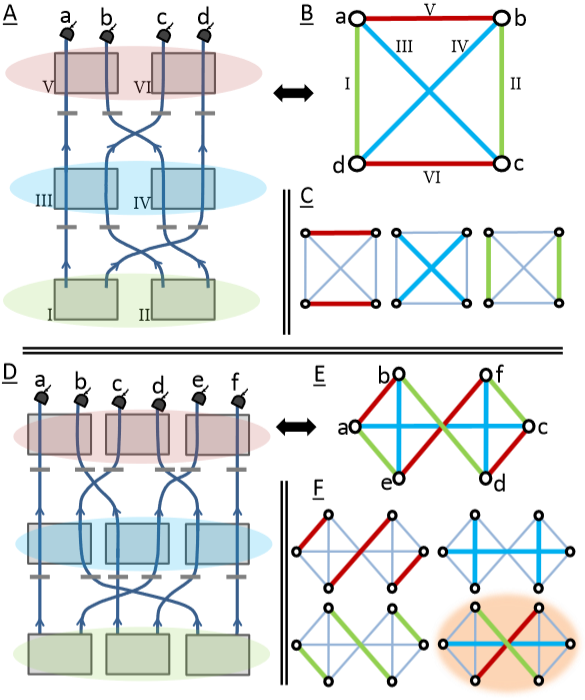
\includegraphics[scale=0.7]{figures/problem_presentation/motivations/krenn_graph.png}
    \caption{This figure was take from Mario Krenn's paper of 2017. \cite{Krenn_2017} It represents 2 examples of experiments to create entangled states using photonic technologies. On one hand, the experiment described in $A$ corresponds to the graph $B$ that is monochromatic as shown in $C$. Therefore, it allows to create a GHZ-state of dimension 3 involving 4 particles $\ket{\psi} = GHZ_{4, 3} = \frac{1}{\sqrt{3}} (\ket{0000} + \ket{1111} + \ket{2222})$. On the other hand, the experiment described in $D$ is represented by the graph in $E$, which is non-monochromatic as shown in $F$. Therefore, the state it creates is not a GHZ-state. $\ket{\psi'} = \frac{1}{2} (\ket{000000} + \ket{111111} + \ket{222222} + \ket{121200})$.}
    \label{fig:krenn_experiment}
\end{figure}

At last, please note that the study of GHZ-states is still very active nowadays. For instance, Alain Aspect, John F. Clauser and Anton Zeilinger received in 2022 a Nobel prize for their experiments on quantum entanglement, and their work was closely related to the topic. \cite{nobelprizeNobelPrize}. Finding new ways to experimentally create such states would open new intriguing gates in the fields of quantum computing \cite{gu2020compact} and cryptography \cite{pivoluska2018layered}.\\
